\documentclass[twoside]{article}
\usepackage{amssymb}
\usepackage{amsthm}
\usepackage{amsmath}
\usepackage{amsfonts}
\usepackage[utf8]{inputenc}
\usepackage[spanish]{babel}
\usepackage{tikz}
\usepackage{centernot}
\usepackage{hyperref}
\usepackage{fancyhdr}
\usepackage{lipsum}
\usepackage{subcaption}
\hypersetup{
    colorlinks,
    citecolor=black,
    filecolor=black,
    linkcolor=black,
    urlcolor=black
}
\usepackage{xurl}
\usepackage[top=1in, bottom=1.5in, left=1in, right=1in]{geometry}
\pagestyle{fancy}
\fancyhead{}
\fancyhead[L]{\leftmark}
\fancyfoot{}
\fancyfoot[C]{\thepage}
\newcommand{\enquote}[1]{``#1''}
\usepackage{float}
\usepackage[parfill]{parskip}
\newcommand{\image}[2]{
\begin{figure}[H]
    \includegraphics[width=#1 cm]{../images/#2.png}
    \centering
\end{figure}
}

\title{Práctica 4 SWAP}
\author{XuSheng Zheng}
\date{}

\begin{document}

\maketitle
\tableofcontents
\newpage

\section{Certificado autoafirmado SSL}
Empezamos habilitando el módulo SSL de Apache y creando el directorio para ubicar los certificados:
\image{8}{1}
Ahora creamos el certificado con los siguientes datos:
\image{8}{2}
\subsection{Opciones avanzadas}
De las opciones introducidas anteriormente, podemos prescindir de \textbf{nodes} para añadir una contraseña a la clave. Además, tenemos las siguientes opciones que pueden ser interesantes:
\begin{itemize}
    \item \textbf{-config filename}: permite especificar un archivo de configuración para la creación de los certificados.
    \item \textbf{-subj arg}: permite especificar datos para la creación del certificado. El argumento debe ser de la forma \textbf{/type0=value0/type1=value1/type2=....}. Al introducir esta opción no nos pedirá los datos como habíamos hecho.
    \item \textbf{-addext ext}: permite añadir una extensión de x509 en el certificado generado.
\end{itemize}
Como ejemplo creamos el siguiente certificado:
\image{8}{5}
Podemos ver que nos pide la contraseña para generar el certificado. Si eliminamos la opción \textbf{-subj} podemos ver que aparte de pedirnos la contraseña nos pide también el resto de informaciones:
\image{8}{6}

\section{Apache con certificado SSL}
Editamos el archivo de configuración \textit{/etc/apache2/sites-available/default-ssl.conf}:
\image{8}{3}
Activamos \textbf{default-ssl} y reiniciamos Apache:
\image{8}{4}
Para comprobar que se ha instalado correctamente el certificado accedemos desde el navegador del anfitrión:
\image{12}{8}
Accedemos al certificado desde el candado con exclamación a la izquierda de la URL:
\image{8}{9}
\image{12}{7}
Ahora procedemos a copiar los archivos que hemos creado anteriormente a m2 y m3:
\image{8}{10}
Al igual que en m1, en m2 creamos el directorio \textit{/etc/apache2/ssl}, copiamos los archivos en dicho directorio y configuramos \textbf{default-ssl}:
\image{8}{11}
\image{8}{12}
\image{8}{13}
Podemos comprobar con \textbf{cURL} que m2 acepta peticiones HTTPS:
\image{8}{14}

\section{Nginx como balanceador para peticiones HTTPS}
En m3 activamos \textbf{Nginx} y aseguramos de que esté en funcionamiento:
\image{8}{15}
Creamos un nuevo directorio \textit{ssl} para guardar los archivos:
\image{8}{16}
Editamos el archivo \textit{/etc/nginx/conf.d/default.conf} para añadir un nuevo bloque \textbf{server} con los siguientes datos:
\image{8}{17}
Reiniciamos \textbf{Nginx} y comprobamos desde el anfitrión:
\image{8}{18}

\subsection{Opciones avanzadas}
A partir de la configuración anterior podemos añadir algunas mejoras. Puesto que las operaciones SSL consume recursos extras del CPU, existen dos maneras de minimizar el número de estas operaciones por cliente: la primera es habilitar la opción \textbf{keepalive} para poder mandar varias peticiones por conexión y la segunda es mediante la reutilización de parámetros de sesión SSL para evitar \textbf{ssl handshakes}. Dichas sesiones se almacenan en un cache que se configura con la directiva \textbf{ssl\_session\_cache}. El timeout por defecto de dicho caché es de 5 minutos, para modificarlo podemos utilizar la directiva \textbf{ssl\_session\_timeout}.

En el siguiente ejemplo habilitamos un cache de tamaño 1MB con un timeout de 10 minutos:
\image{8}{19}



\begin{figure}[H]
    \centering
    \begin{subfigure}{.5\textwidth}
        \centering
%        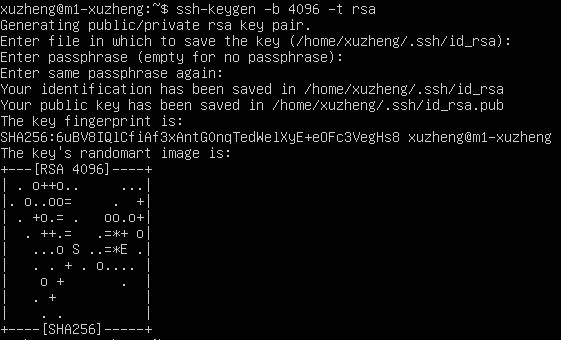
\includegraphics[width=7cm]{../images/13.png}
    \end{subfigure}%
    \begin{subfigure}{.5\textwidth}
        \centering
%        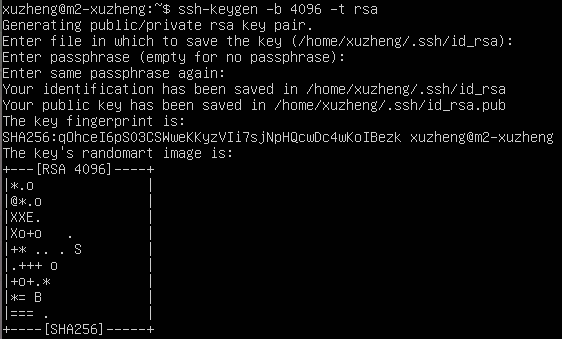
\includegraphics[width=7cm]{../images/14.png}
    \end{subfigure}
\end{figure}


\newpage
\section{Bibliografía}
\begin{itemize}
    \item \url{https://www.openssl.org/docs/manmaster/man1/openssl-req.html}
    

    \item \url{https://linux.die.net/man/1/tar}
    \item \url{https://serverfault.com/questions/141773/what-is-archive-mode-in-rsync}
    \item \url{https://ss64.com/bash/rsync.html}
    \item \url{https://linux.die.net/man/1/rsync}
    \item \url{https://serverfault.com/questions/123629/run-task-every-90-minutes-with-cron}
\end{itemize}

\end{document}
